\section{Trabalhos relacionados}\label{sec:trabalhos}

Nesta seção apresentaremos a API webaudio e as ferramentas / frameworks Gibber e Wavepot.

\subsection*{WebAudio API}\label{sec:webaudioapi}

O primeiro trabalho relacionado é a própria API Webaudio e seu nó especial para processamento de sinais (\emph{ScriptProcessorNode}), que permite os três trabalhos serem co-relacionados.
Uma característica lógica do ScriptProcessorNode é sua linearidade, possibilitando calcular cada amostra do vetor de saída de maneira direta.
Isto permite \begin{inparaenum}[\itshape a)\upshape]
\item uma possível redução no custo  computacional para sínteses de ondas complexas;
\item a definição matemática de um vetor de saída a partir da definição de uma função; e
\item a criação de qualquer tipo de nó de processamento de áudio\end{inparaenum}.
No Código \ref{code:ex1} demonstramos uma simples utilização desta API.

\begin{listing}
\begin{minted}[linenos,frame=lines,framesep=2mm,fontsize=\scriptsize]{javascript}
// Chrome ou firefox?
var context = new AudioContext();
var node = context.createScriptProcessor(1024, 0, 1);

// DSP
var noise = function(amplitude){
    var sample = Math.random() * 2 - 1
    return sample * amplitude
}

node.onaudioprocess = function(e) {
  var output = e.outputBuffer.getChannelData(0);
  for (var i = 0; i < data.length; ++i) {
    output[i] = noise(0.5)
  }
}
node.connect(context.destination); // TOCAR
node.disconnect(); // PARAR
\end{minted}
\caption{Exemplo de utilização do ScriptProcessorNode}
\label{code:ex1}
\end{listing}

Esta abordagem é conveniente do posto de vista musical entre as linhas e 6-9 do Código \ref{code:ex1}. Para o músico, o restante pode ser  especificidade técnica que pode desviar a atenção composicional. Nesse sentido, o \emph{Gibber} e \emph{Wavepot} oferecem soluções possíveis para aqueles que se interessam em manter um controle dos algoritmos musicais.

% http://lammax.lnu.se/ubimus/wp-content/uploads/sites/5/2015/03/ubimus6_submission_2.pdf
% -----------------------------------------------
% -----------------------------------------------
% -----------------------------------------------
% -----------------------------------------------
% -----------------------------------------------
% -----------------------------------------------
% -----------------------------------------------
\subsection*{Gibber}

O Gibber\footnote{Disponível em \url{http://gibber.mat.ucsb.edu/}.} é descrito por \cite{roberts_gibber:_2012} como um ambiente de \emph{live coding}\footnote{Para mais informações sobre a prática \emph{live coding}, sugerimos a leitura dos seguintes autores: \cite{collins_live_2003,ward_live_2004,collins_live_2007,rohrhuber_improvising_2009,magnusson_algorithms_2011,collins_origins_2014}. Seu foco está em tornar a atividade de codificação produtiva do ponto de vista musical.}. Possui um \emph{layout} de abas divididas entre: \begin{inparaenum}[\itshape 1)\upshape]
\item editor de texto;
\item um \emph{canvas} contendo imagens resultantes dos códigos visuais;
\item um navegador do aplicativo, contendo rotinas diversas;
\item alternador de códigos sonoros e códigos visuais
\item navegador de códigos musicais do servidor;
\item um console de informações;
\item \emph{login} para um círculo de contas restritas ao aplicativo.
\end{inparaenum}Nosso interesse maior tange ao item 1, e em como o código escrito processa os sinais digitais.Uma outra abordagem técnica, descrita na próxima sessão,  elucida as linhas 136-175 do código-fonte da máquina de áudio do \emph{Gibber}, \emph{Gibberish}\footnote{Disponível em \url{https://github.com/charlieroberts/Gibberish}.}. Descartaremos portanto o estudo do \emph{Gibber} para focar no \emph{Wavepot}.

\begin{figure}[h]
\centering
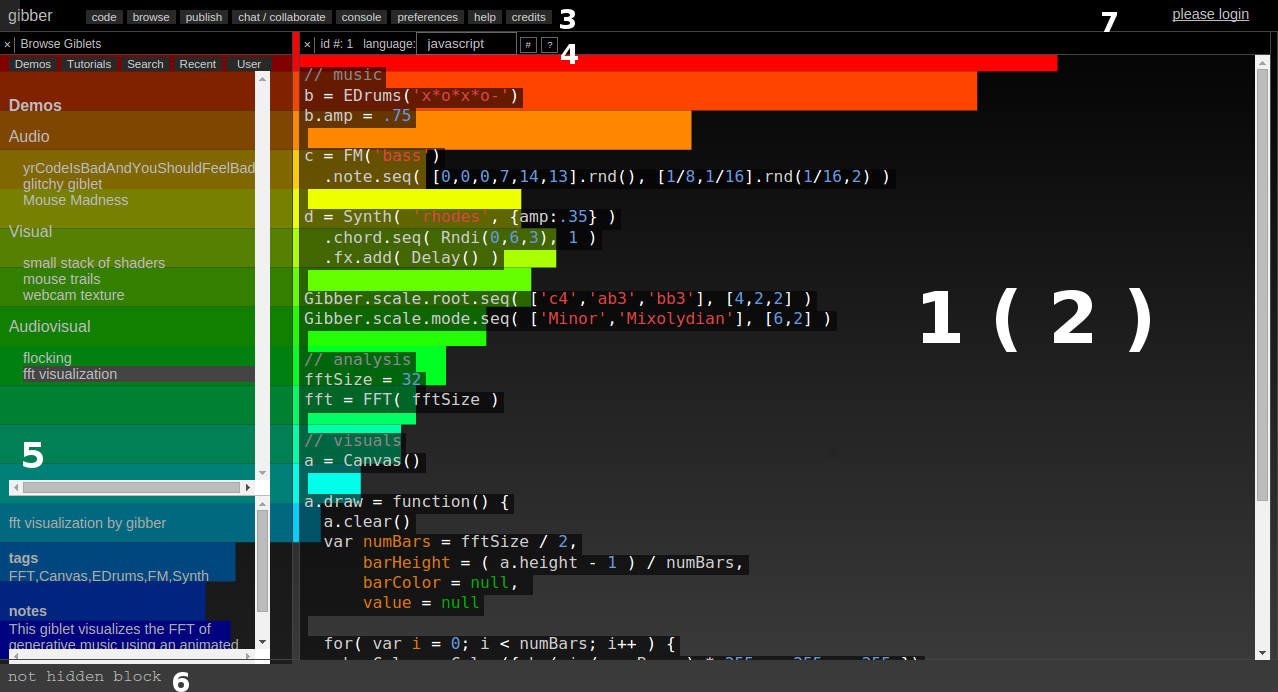
\includegraphics[scale=0.35]{gibber.png}
\caption{Aplicativo \emph{Gibber}. \textbf{Fonte}: \protect\url{http://gibber.mat.ucsb.edu}}
\label{fig:gibber}
\end{figure}


% -----------------------------------------------
% -----------------------------------------------
% -----------------------------------------------
% -----------------------------------------------
% -----------------------------------------------
% -----------------------------------------------
% -----------------------------------------------
\subsection*{Wavepot}

É uma \emph{webaudio-daw}\footnote{\emph{Webaudio Digital Audio Workstation} disponível em \url{https://github.com/wavepot/wavep0t/blob/master/index.js}.}.
Esta ferramenta possui as seguintes características:\begin{inparaenum}[\itshape 1)\upshape]
\item layout que expõe a partitura-programação \cite{fenerich_marulho_2014} do lado esquerdo. Geralmente é dividida em dois editores, semelhante ao método \emph{instrumento-orquestra}~\cite{mathews_digital_1963,di_nunzio_genesi_2010};
\item do lado direito, controles de tocar, parar e gravar, menu de exemplos, módulos, músicas, ajuda, alternáveis;
\item compartilhamento e atualizações dos códigos através do \emph{Github};
\item um analisador gráfico da formas de onda resultantes;
\item uma lista de cabeçalhos dos códigos abertos;
\item um console de retorno de informações.
\end{inparaenum}

\begin{figure}[h]
\centering
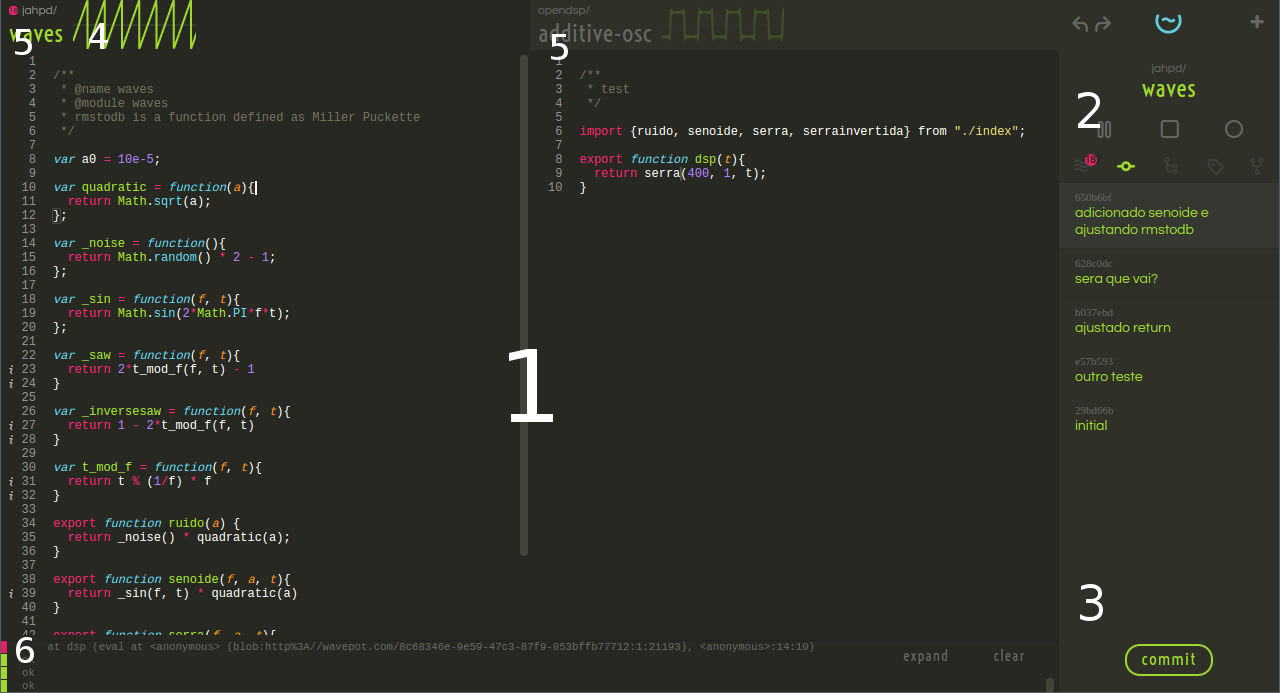
\includegraphics[scale=0.35]{wavepot.png}
\caption{Aplicativo \emph{Wavepot}. \textbf{Fonte}: \protect\url{https://www.wavepot.com}}
\label{fig:wavepot}
\end{figure}

Existe um modo padronizado de programação que requer observações. A primeira é que o improvisador utilize uma variável $t$. Esta variável pode ser descrita como a fase de um tempo discretizado $td=1/sampleRate$. É util para calcular formas de ondas diversas. No exemplo \ref{code:ex2} demonstramos o uso do $t$ para criar uma senóide. A segunda exige a utilização do \emph{token} \verb|export| antes de definir a função $dsp$.


\begin{listing}
\begin{minted}[linenos,frame=lines,framesep=2mm,fontsize=\scriptsize]{javascript}
var noise = function(amplitude){
    return (Math.random() * 2 - 1) * a;
}

var sin = function(freq, amp, t){
    return Math.sin(Math.PI * 2 * freq * t) * a
}

export function dsp(t){
    return noise(1) * sin(1, 1, t)
}
\end{minted}
\caption{Sintetizando um ruído controlado por um LFO senoidal}
\label{code:ex2}
\end{listing}

% -----------------------------------------------


\subsection{Comparação de trabalhos relacionados}

Para entender a relação entre estas duas ferramentas, montamos um quadro comparativo a partir de alguns parâmetros: tipo de música realizada nos códigos exemplares,  suporte a vídeo, compilação em tempo de execução, estratégia de partitura-programação,  biblioteca de síntese e suporte ao compartilhamento dos códigos. Esta comparação é apresentada na Tabela \ref{tab:comparacao}.
Em ambos os casos, ocorre a tradução de um código em linguagem \emph{javascript} para o processamento de áudio.
Uma discussão musicológica envolve entre outros fatores, um tipo de música tocado em eventos conhecidos como \emph{algoraves}~\cite{collins_algorave:_2014,mori_analysing_2015}.

\renewcommand{\arraystretch}{1.35} %Espacamento entre as linhas

\begin{table}[ht!]
\caption{Tabela comparativa de funcionalidades entre o \emph{Gibber} e o \emph{Wavepot}.}
    \begin{tabular}{ p{4cm} | p{5cm} | p{5cm}}
    \hline 
    \hline 
    \textbf{Característica}      & \textbf{Wavepot}  & \textbf{Gibber} \\
    \hline 
    \hline 
    
    Linguagem de programação & Javascript & Javascript \\
    \hline
    
    Tipo de música      & Algorave & Algorave + glitch/noise\\
    \hline
    
    Vídeo               & Não      & \small Sim - Síntese de imagens 2D e 3D através de uma implementação OpenGL. Podem sincronizar com alguns parâmetros sonoros.    \\
    \hline
    
    Compilação em tempo de execução & \small Sim -- qualquer edição no código é automaticamente reconhecido enquanto estiver sendo processado algum sinal de áudio. & \small Sim -- o executante musical deve utilizar teclas de atalho para requerir ao servidor o processo de compilação. \\
    \hline
    
    Partitura-programação      & \small Editor de texto desenvolvido com a biblioteca \emph{Ace}\footnotemark \footnote{Disponível em \url{http://ace.c9.io/#nav=about}.} em duas partes, subdividido pelos autores deste artigo como \emph{instrumentais} e \emph{orquestrais}  & \small Editor de texto, com alternância dos códigos sonoros (\emph{javascript}) e códigos visuais (\emph{OpenGL}) \\
    \hline

    Biblioteca de síntese  & 
    $Audio-process$\footnote{Disponível em \url{https://github.com/wavepot/wavep0t/blob/master/index.js}.} & 
    Gibberish\footnote{Disponível em \url{https://github.com/charlieroberts/Gibberish/blob/master/scripts/gibberish.js}.}    \\
    \hline
    
    Criação de novos módulos em tempo de execução  & \small Sim -- o improvisador pode criar funções através de variáveis ou as palavras-chave $export default function$ & Não \\
    \hline
    Compartilhamento de códigos &
    O usuário pode criar, ou reutilizar módulos e músicas, através da rede social $Github$  & 
    Códigos musicais podem ser publicados no servidor do Gibber abrindo uma conta no próprio site. \\
    \hline 
    Elementos de GUI &
    \small Não existe na versão oficial, no entanto um experimento foi desenvolvido para sincronizar a máquina de síntese \emph{Wavepot} com controladores MIDI\footnote{A discussão inteira está disponível em \url{https://groups.google.com/forum/?hl=pt-BR#!topic/wavepot/i5H7rRvcdpQ}, enquanto o exemplo está disponível em \url{http://boxbase.org/sequencer/}.}. A GUI servia, portanto, para averiguar o funcionamento do MIDI.  &
    Sim -- Pode ser utilizado com a biblioteca \emph{Interface.js}\footnote{} \\
    \hline
    \hline
    \end{tabular}
\label{tab:comparacao}
\end{table}


%Enquanto o primeiro possui um código aberto desde 16 de Junho de 2012\footnote{Disponível em \url{https://github.com/charlieroberts/Gibberish/commit/fec69715908505869e6fa8e7fca4e5eb08ea1f4e}.}, o segundo abriu parcialmente o código no começo de Setembro\footnote{Disponível em \url{https://github.com/wavepot/wavep0t/commit/ed988a9512bb5244b500cfbbeae77f94741856c5}.}